\section{Visuelle detaljer}


\subsection{Ikoner}
Figur \ref{fig:appikoner} presenterer alle aplikasjonsikoner som brukes til vinduer i programmet. Alle ikoner til subvinduer er satt sammen av vår egen ikone og "<open source"> ikoner (se \ref{subssec:utvmiljo}, side \pageref{subssec:utvmiljo}). Hensikten med slike kompositikoner er at de skal gi en mer visuell tilbakeleding til brukeren som viser hvilken aktuelle funksjon som so brukes i programmet. 

\begin{figure}[ht!]
\centering
\begin{subfigure}[b]{0.2\textwidth}
\centering

\includegraphics[scale=0.4]{./img/produktdokumentasjon/visuelle_detaljer/boligLogo.png}
\caption{Programikone}
\end{subfigure}
\quad
\begin{subfigure}[b]{0.2\textwidth}
\centering

\includegraphics[scale=0.4]{./img/produktdokumentasjon/visuelle_detaljer/ny_bolig.png}
\caption{Ny bolig}
\end{subfigure}
\quad
\begin{subfigure}[b]{0.2\textwidth}
\centering

\includegraphics[scale=0.4]{./img/produktdokumentasjon/visuelle_detaljer/ny_utleier.png}
\caption{Ny utleier}
\end{subfigure}
\quad
\begin{subfigure}[b]{0.2\textwidth}
\centering

\includegraphics[scale=0.4]{./img/produktdokumentasjon/visuelle_detaljer/edit.png}
\caption{Endre}
\end{subfigure}
\quad
\begin{subfigure}[b]{0.2\textwidth}
\centering

\includegraphics[scale=0.4]{./img/produktdokumentasjon/visuelle_detaljer/foresporsel.png}
\caption{Forespørsel}
\end{subfigure}
\quad
\begin{subfigure}[b]{0.2\textwidth}
\centering

\includegraphics[scale=0.4]{./img/produktdokumentasjon/visuelle_detaljer/bildevindu.png}
\caption{Bilder}
\end{subfigure}
\quad
\begin{subfigure}[b]{0.2\textwidth}
\centering

\includegraphics[scale=0.4]{./img/produktdokumentasjon/visuelle_detaljer/passord.png}
\caption{Pålogging}
\end{subfigure}
\quad
\caption{Applikasjons og vinduikoner}\label{fig:appikoner}
\end{figure}


\subsection{Presentasjon}
Figur \ref{fig:presentasjon} viser eksepel på hvordan objektene vises i \texttt{JEditorPane} gjennom html visning. Datafelt for objektet pareses i klassen \texttt{ControllerOutput.java} i en metodene som er tilpasset til visning av spesifkk objekt, f.eks boligobjektene vises gjennom \texttt{visBoligObjektHTMLOutput(Object valgtObjekt, JEditorPane output, AbstraktArkfane vindu, HashSet<Bolig> boligliste)}. Det er noen begrensninger i forhold til html visningen da \texttt{JEditorPane} er kun kapabel til visning av Html versjon 3.2 og CSS 1.0 (release fra år 1997). 

\begin{figure}[ht!]
 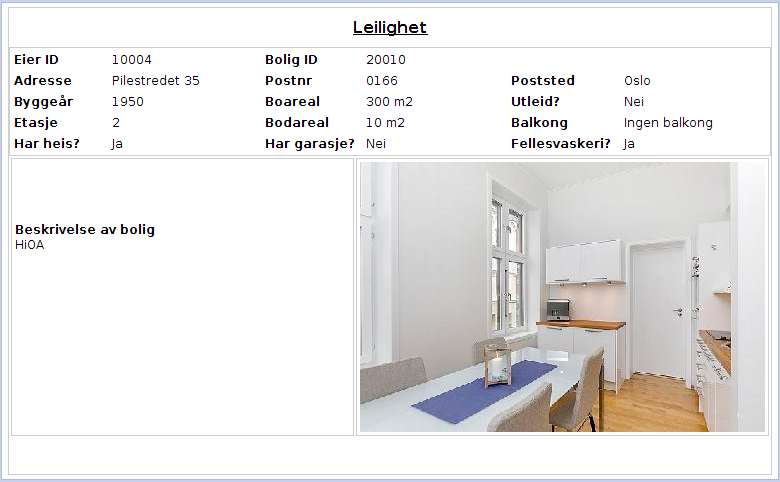
\includegraphics[width=\textwidth,height=\textheight,keepaspectratio]{./img/produktdokumentasjon/visuelle_detaljer/presentasjon.png}
 \caption{HTML presentasjon av et boligobjekt.}
 \label{fig:presentasjon}
\end{figure}


\subsection{Tabell}
I figur \ref{fig:tabell} presenteres utseende på formatert tabellobjekt, der annenhver rad har en annen bagrunnfarve og får en tredje bakgrunfarve ved markering. Forskejllige farver brukes i tilleg til horisontelle linjer med hensikt å oppnå en bedre avskilt linje mellom presentasjonen av tabellkomponenter. Alle tabeller i programmet har også innkludert en meny som hører til de forskjellige obejktene utefra hvilke fubnkjsoner i programmet som kan brukes på et vist objekt. For eksepel i en tabell over boligobjekter, for boligobjektene kan man endre, slette eller endre publiseringsstatus. Dersom brukeren skriver ut innhold i utleierregisteret vil det blir presentert alternativer som er spesifikke for objekter som instasierer superklassen person (ny endre, slett) men i tilleg funksjoner som er spesifikke for klassen utleier (som presentert i den refererte figuren). I eksemplet har vi mulighet at gjennom å markere en person direkte gå til registreringsdialog for bolig som kan registreres på den personen. Vi kan også editere boliger som tilhører denne eieren eller også slette dem. Sammen funkjsonalitet er også da tilgjengelig via den vanlige og synlige gui komponenter som knapper eller også gjennom å dobbelklikker i tabellen.

\begin{figure}[ht!]
\center
 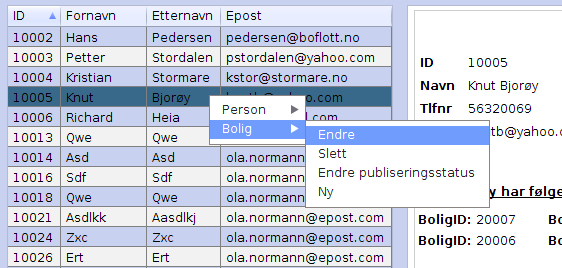
\includegraphics[scale=0.7]{./img/produktdokumentasjon/visuelle_detaljer/tabell.png}
 \caption{Visning og markering i tabell}
 \label{fig:tabell}
\end{figure}

\subsection{Grafisk tema}
Med hensikt å få bedre portabilitet mellom forskjellige operativsystem har standard Java "<LookAndFeel"> endret fra \texttt{Metal} til det nyeste swing tema \texttt{Nimbus}. Den primære årsaken til dette er at det ble observert noen forskjeller på størrelse og layout av gui komponenter mellom operativsystemene som programmet var testet på. Eksepelvis dersom programmet testedes i Linux miljør finns det ingen "<native"> grafisk miljø i form av komponenter som knapper men på OS der Java er kapabel å renderere stadrad kanpper for systemet ble det noen forskjeller mellom slike komponenter\footnote{Etter tester på Mac OS og Windows.}. Bruk av nimbus som primær tema for gui komponenter gir sikkerhet at alle kompoenentene kommer til å bli renderert gjennom JVM hvilket gir en god portabilitet mellom operativsystemene. 

REFERER HER TIL AVSNITTET OM PORTABILITET


\begin{figure}[ht!]
\centering
\begin{subfigure}[b]{0.4\textwidth}
\centering
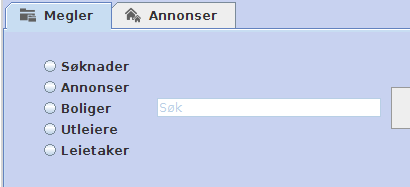
\includegraphics[scale=0.5]{./img/produktdokumentasjon/visuelle_detaljer/metal.png}
\caption{Stadard tema "<metal">}
\end{subfigure}

\begin{subfigure}[b]{0.4\textwidth}
\centering
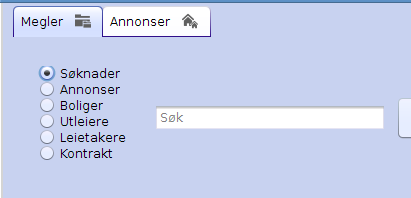
\includegraphics[scale=0.5]{./img/produktdokumentasjon/visuelle_detaljer/nimbus.png}
\caption{Nimbus}
\end{subfigure}
\caption{Applikasjons og vinduikoner}\label{fig:tema}
\end{figure}